\subsection{Simulation Analysis}

\begin{tcolorbox}	
\begin{tabular}{p{2.75cm} p{0.2cm} p{10.5cm}}
\textbf{Contributors}  &:& Diamantino Silva, (2017-08-18 - ...)\\
\textbf{Goal}          &:& Simulation of various optical detection schemes.\\
\textbf{Directory}     &:& sdf/optical\_detection
\end{tabular}
\end{tcolorbox}
%
\vspace{2em}
%



\begin{figure}[H]
\centering
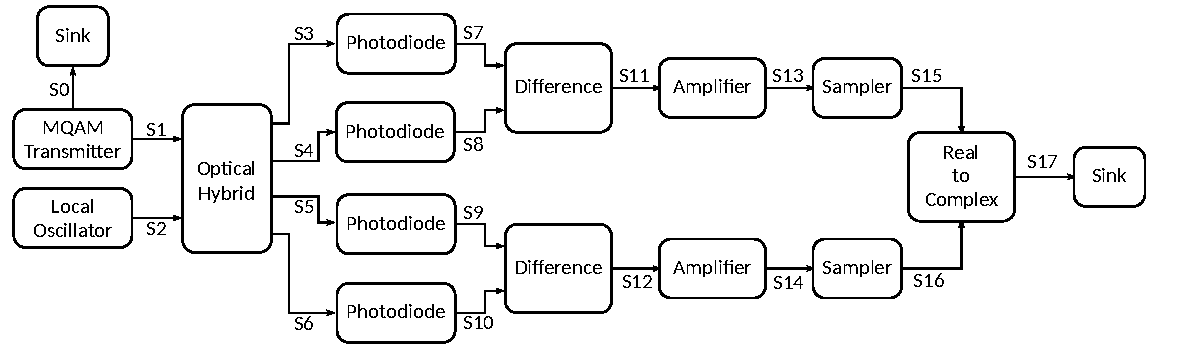
\includegraphics[width=\linewidth]{./sdf/optical_detection/figures/scheme_setup.pdf}
\caption{Overview of the simulated optical system.}
\label{fig:setup}
\end{figure}
%
\vspace{1em}
%
List of signals used in the simulation:
\begin{table}[H]
\centering
\begin{tabular}{|c|l|l|}
\hline
\bf{Signal name}	& \bf{Signal type}						& \bf{Status}\\
\hline
S0					& Binary								& check\\
S1					& OpticalSignal							& check\\
S2					& OpticalSignal							& check\\
S3					& OpticalSignal							& check\\
S4					& OpticalSignal							& check\\
S5					& OpticalSignal							& check\\
S6					& OpticalSignal							& check\\
S7					& TimeContinuousAmplitudeContinuousReal	& check\\
S8					& TimeContinuousAmplitudeContinuousReal	& check\\
S9					& TimeContinuousAmplitudeContinuousReal	& check\\
S10					& TimeContinuousAmplitudeContinuousReal	& check\\
S11					& TimeContinuousAmplitudeContinuousReal	& check\\
S12					& TimeContinuousAmplitudeContinuousReal	& check\\
S13					& TimeContinuousAmplitudeContinuousReal	& check\\
S14					& TimeContinuousAmplitudeContinuousReal	& check\\
S15					& TimeDiscreteAmplitudeContinuousReal	& check\\
S16					& TimeDiscreteAmplitudeContinuousReal	& check\\
S17					& OpticalSignal							& check\\
\hline
\end{tabular}
\end{table}
%
\vspace{2em}
%
This system takes into account the following input parameters:
\begin{table}[H]
\centering
\begin{tabulary}{1.0\textwidth}{|c|p{30mm}|p{70mm}|}
\hline
\textbf{System Parameters}	& {\bf Default value}		& \textbf{Description}\\
\hline
localOscillatorPower1		& $2.0505 \times 10^{-8}$W	& Sets the optical power, in units of W, of the local oscillator inside the MQAM\\
\hline
localOscillatorPower2		& $2.0505 \times 10^{-8}$W	& Sets the optical power, in units of W, of the local oscillator used for Bob's measurements\\
\hline
localOscillatorPhase		& $0$ rad					& Sets the initial phase of the local oscillator used in the detection\\
\hline
responsivity				& $1$ A/W					& Sets the responsivity of the photodiodes used in the homodyne detectors\\
\hline
iqAmplitudeValues			& $\{ \{ 1, 1 \}, \{ -1, 1 \},$ $ \{ -1, -1 \}, \{ 1, -1 \} \}$
														& Sets the amplitude of the states used in the MQAM\\
%
%\hline
%transferMatrix				&
%							$\frac{1}{\sqrt{2}}\{1,1,1,1\}$	
%							& Sets the transfer matrix of the beam splitter used in the homodyne detector\\
%\hline
%shotNoise (FUTURE)      & Chooses if quantum shot noise is used in the simulation\\
%\hline
%thermalNoise (FUTURE)   & Chooses if thermal noise is used in the simulation\\
%\hline
%thermalNoiseAmplitude  (FUTURE)  & Sets the amplitude of the thermal noise\\
%
\hline
\end{tabulary}
\end{table}
%
\vspace{2em}
%
The simulation setup is represented in figure \ref{fig:setup}. The starting point is the MQAM, which generates random states from the constelation given by the variable \texttt{iqAmplitudeValues}. The output from the generator is received in the Optical Hybrid where it is mixed with a local oscillator, outputing two optical signal pairs. Each pair is converted to currents by two photodiodes, and the same currents are subtracted from each other, originating another current proportional to one of the quadratures of the input state.
The other pair suffers the same process, but the resulting subtraction current will be proportional to another quadrature, dephased by $\pi/2$ relative to the other quadrature.\\
%
%\begin{table}[H]
%\centering
%\begin{tabular}{c|c}
%System Blocks                         & netxpto Blocks\\
%\hline
%M - Quadrature Amplitude Modulator    & MQamTransmitter\\
%Local Oscillator                      & LocalOscillator\\
%90deg Optical Hybrid                  & OpticalHybrid\\
%Photodiode                            & Photodiode\\
%Difference Circuit                    & Difference\\
%Sampler                               & Sampler\\
%\end{tabular}
%\end{table}


\subsection*{Required files}\label{Required files}

Header Files
\begin{table}[H]
\centering
\begin{tabulary}{1.0\textwidth}{|L|L|l|}
\hline
\textbf{File}			& \textbf{Description}									& {\bf Status}\\
\hline
netxpto.h               & Generic purpose simulator definitions.				& check\\
\hline
m\_qam\_transmitter.h   & Outputs a QPSK modulated optical signal.				& check\\
\hline
local\_oscillator.h     & Generates continuous coherent signal.					& check\\
\hline
optical\_hybrid.h       & Mixes the two input signals into four outputs.		& check\\
\hline
photodiode.h            & Converts an optical signal to a current.				& check\\
\hline
difference.h            & Ouputs the difference between two input signals.		& check\\
\hline
ideal\_amplifier.h		& Performs a perfect amplification of the input sinal	& check\\
\hline
sampler.h               & Samples the input signal.								& check\\
\hline
real\_to\_complex.h		& Combines two real input signals into a complex signal	& check\\
\hline
sink.h                  & Closes any unused signals.							& check\\
\hline
\end{tabulary}
\end{table}
%
%
Source Files
\begin{table}[H]
\centering
\begin{tabulary}{1.0\textwidth}{|L|L|l|}
\hline
\textbf{File}			& \textbf{Description}									& {\bf Status}\\
\hline
netxpto.cpp				& Generic purpose simulator definitions.				& check\\
\hline
m\_qam\_transmitter.cpp	& Outputs a QPSK modulated optical signal.				& check\\
\hline
local\_oscillator.cpp	& Generates continuous coherent signal.					& check\\
\hline
optical\_hybrid.cpp		& Mixes the two input signals into four outputs.		& check\\
\hline
photodiode.h			& Converts an optical signal to a current.				& check\\
\hline
difference.h			& Ouputs the difference between two input signals.		& check\\
\hline
ideal\_amplifier.h		& Performs a perfect amplification of the input sinal	& check\\
\hline
sampler.cpp				& Samples the input signal.								& check\\
\hline
real\_to\_complex.cpp	& Combines two real input signals into a complex signal	& check\\
\hline
sink.cpp				& Empties the signal buffer.							& check\\
\hline
\end{tabulary}
\end{table}



%\subsection*{Inputs}

%This system takes no inputs.

%\pagebreak
%\subsection*{Outputs}

%The system outputs the following objects:
%\begin{itemize}
%\item Signals:
%\begin{itemize}
%\item Binary Sequence used in the MQAM; (S$_{0}$)
%\item Local Oscillator used in the MQAM; (S$_{1}$)
%\item Local Oscillator used in the detection; (S$_{2}$)
%\item Optical Hybrid Outputs; (S$_{3}$, S$_{4}$, S$_{5}$, S$_{6}$)
%\item In phase Photodiodes output; (S$_{7}$, S$_{8}$)
%\item Quadrature Photodiode output; (S$_{9}$, S$_{10}$)
%\item In phase Difference output; (S$_{11}$)
%\item Quadrature Difference output; (S$_{12}$)
%\item In phase Sampler output; (S$_{13}$)
%\item Quadrature Sampler output; (S$_{14}$)
%\end{itemize}
%\end{itemize}


\pagebreak


\subsection*{Simulation Results}\label{subsec:SHresults}

To test the simulated implementation, a series of states $\{\ket{\phi_i}\}$ were generated and detected, resulting in a series of measurements $\{(x_i,y_i)\}$. The simulation result is presented in figure $\ref{fig:constelation}$:
%
\begin{figure}[H]
\centering
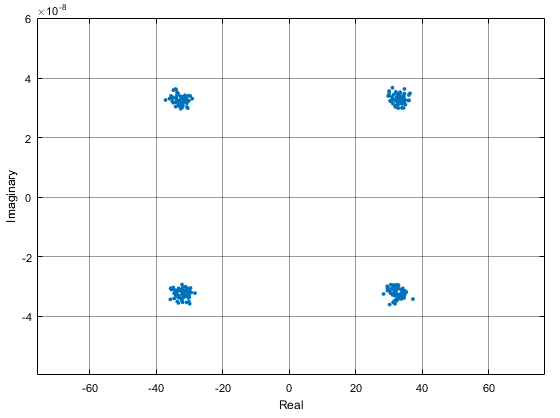
\includegraphics[width=10cm]{./sdf/optical_detection/figures/constelation1.png}
\caption{Simulation of a constelation of 4 states (n = 100)}
\label{fig:constelation}
\end{figure}
%
We see that the measurements made groups in certain regions. Each of this groups is centered in the expected value $(\braket{\textrm{X}}, \braket{\textrm{Y}})$ of one the generated states. Also, they show some variance, which was tested for various expected number of photons, $\braket{n}$, resulting in figure \ref{fig:variance}:
%
\begin{figure}[H]
\captionsetup{justification=centering}
\centering
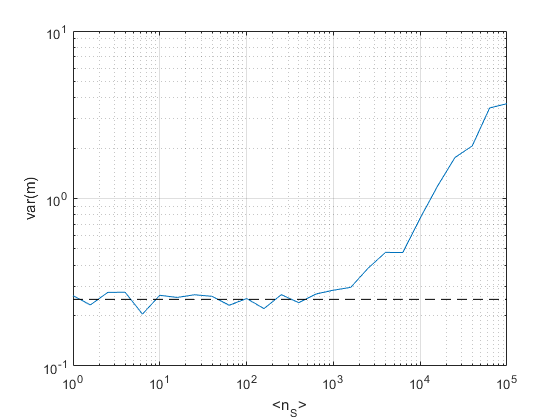
\includegraphics[width=10cm]{./sdf/optical_detection/figures/plot_var_vs_n1.png}
\caption{Simulation of the variance of $m$.\\Local oscillator expected number of photons: $10^4$}
\label{fig:variance}
\end{figure}
%
It was expected that the variance should independent of the input's signal number of photons. Plot \ref{fig:variance} shows that for low values of $n_S$, the simulation is in accordance with the theoretical prevision, with $\textrm{Var(X)} = \textrm{Var(Y)} = \frac{1}{4}$ . For large values of $n_S$, when the number of photons is about the same has the local oscillator, the quantum noise variance starts to grow proportionally to $n_S$, in accordance with the non approximated calculation of quantum noise (eq. \ref{eq:noise}).\\
\\
{\bf Noise Variance with LO power Simulation}\\
The following plot shows the behavior of current noise variance $\braket{(\Delta i)^2}$ with local oscilator power, $P_{LO}$:
%
%
\begin{figure}[H]
	\centering
	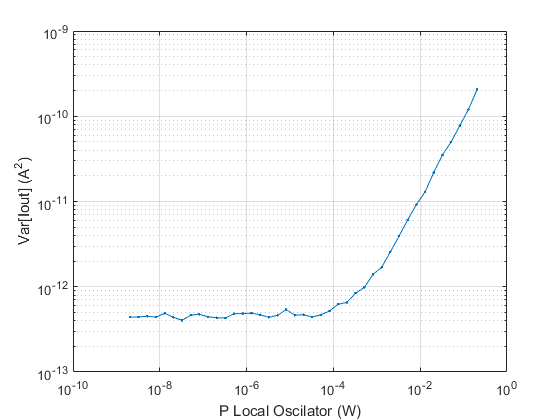
\includegraphics[width=10cm]{./sdf/optical_detection/figures/power_plot.png}
	\caption{Output current variance in function of LO power.}
	\label{fig:variance_lo_power}
\end{figure}
%
%
We see that for low LO power, the dominant noise is the thermal contribution, but for higher power, quantum noise dominates, growing proportionally to $P_{LO}$. This in accordance with equation \ref{eq:var_m}\\
%
%
%
%